\documentclass[../../main.tex]{subfiles}

\graphicspath{{../../fig/}}
\setcounter{section}{0}

\begin{document}

\chapter{ワイヤーのたわみ量評価系の開発と、自動化手法の確立}
\label{chap:wiresag}
較正に使う直線偏光はワイヤーに沿う形で生成されるため、ワイヤーがたわんでいる部分から生成される光はその偏光角が
ワイヤーに沿う方向からずれて生成される。そのため、ワイヤーのたわみは較正の精度に影響を及ぼし、系統誤差を生む。
\ref{subsec:wg_wiresag}項では、過去に行われた評価手法について述べ、この手法にはいくつかの問題があった。
本章では、初めにこの問題について今一度触れたあと、それを解決するために開発したワイヤーのたわみを評価する系について述べる。
その後、評価系の性能評価を行い、最後に実際にスパースワイヤーグリッドに対して行った評価結果について述べる。

\section{過去の測定手法における問題点と開発目標}
\colortext{blue}{過去の測定手法についてもう一度 review するべきか、
それとも\ref{subsec:wg_wiresag}項をもっと簡素にし、詳細な内容をこちらに持ってくるべきか、
現在のようにrefするだけにするべきか悩んでいる。}

過去の測定手法については、\ref{subsec:wg_wiresag}項にて述べたとおりであり、その手法にはいくつかの問題点があった。
一つ目の問題点は、その測定精度が低いことである。これはたわみ量の系統誤差への寄与を必要以上に大きくしている。
また、図\ref{fig:wiresag_result_old}にて示されているように、
全てのワイヤーに対してそのたわみ量は期待される量からどの程度外れているかを判別できておらず、
品質の低いワイヤーを選別できていない。
もう一つの問題点は、その測定手法が人力にて行われており、測定のために労力と時間がかかる点である。
これによりスパースワイヤーグリッドの量産、品質の保証・管理のために繰り返し測定することが困難である。
また、人力での測定はその測定結果に人依存のバイアスを産む可能性がある。

以上の問題点を解決するため、
\begin{enumerate}
    \item ワイヤーのたわみ量 $\order{0.01\tcdegree}$ の精度で評価可能であること
    \item 全てのワイヤーのたわみ量を自動的に評価可能であること
\end{enumerate}
という2点の開発目標をもって新たなワイヤーのたわみ量の評価系を開発した。

\section{評価原理と評価系の設計}

図\ref{fig:wiresag_system}に開発し、組み上げた評価系の概観を示す。


\begin{figure}
    \centering
    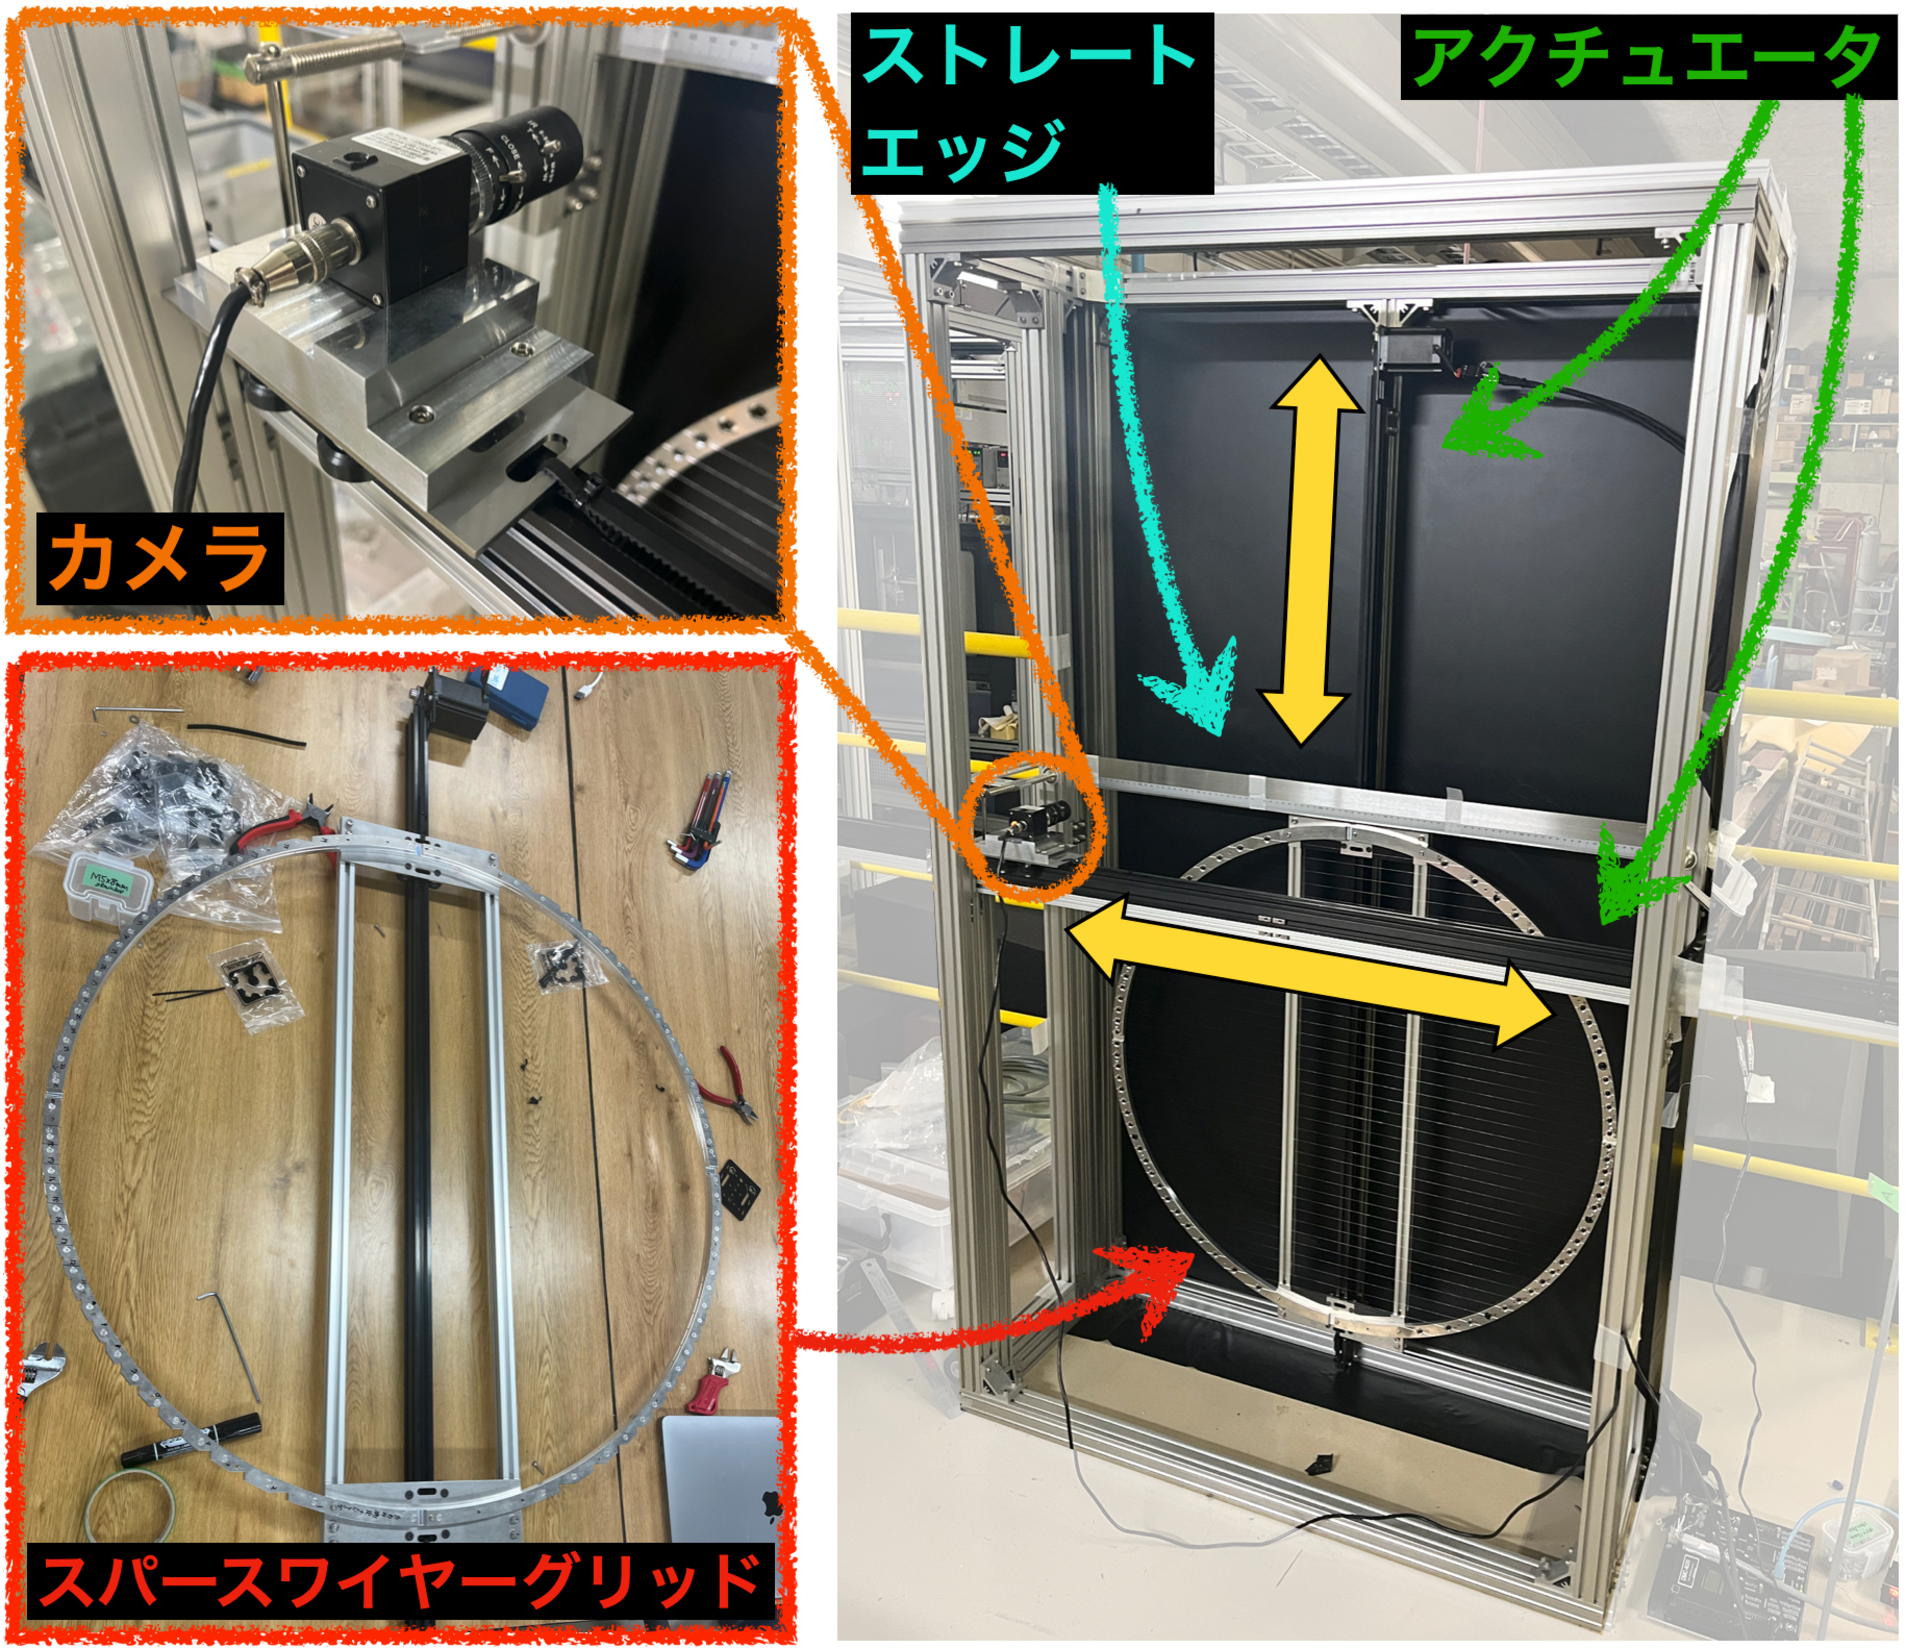
\includegraphics[width=0.8\textwidth]{wiresag/wiresag_system.pdf}
    \caption{ワイヤーのたわみ量評価系の概観}
    \label{fig:wiresag_system}
\end{figure}


\section{解析手法}

\section{開発した評価系のパフォーマンスチェック}

\section{スパースワイヤーグリッドのたわみ量の評価}

\end{document}